\documentclass[11pt,letterpaper,conference]{IEEEtran}

\listfiles
\usepackage{fontspec}
% \usepackage{amsmath}
% \usepackage[mathrm=sym]{unicode-math}
\usepackage[mathrm=sym, warnings-off={
    mathtools-colon,mathtools-overbracket}]{unicode-math}
\setmainfont{Arial}
\setsansfont{Arial}
\setmonofont{MonoLisa}
\setmathfont{FiraMath-Regular.otf}


\input{_preamble/preamble_letter.tex}
\input{_preamble/preamble_float.tex}
\input{_preamble/preamble_units.tex}
\input{_preamble/preamble_table.tex}

\usepackage[export]{adjustbox}

\usepackage{caption}
\usepackage{balance}

\usepackage[backend=biber,      % replace bibtex with biber (bibliography backend engine)
    bibstyle=ieee,              % write literature lists in IEEE style
    citestyle=numeric-comp,     % \cite uses a numeric key
    sortcites=true,
    maxbibnames=3
]{biblatex}
\addbibresource{references.bib}

\usepackage{listings}
\lstset{
    basicstyle = \ttfamily,
    xleftmargin = 1cm,
    frame = single,
    framesep = 1cm,
    numbers = left,
    numbersep = 1.25cm,
    breaklines = true,
    upquote = true
}
\usepackage{titling}
\usepackage{subfiles}

\setlength\parindent{0.25in}

%% DOCUMENT %%%
\begin{document}
\begin{titlepage}
    \begin{minipage}[t]{0.45\textwidth}
        \begin{flushleft}
            
\includegraphics[valign=t,width=\textwidth]{images/wsu.png}
        \end{flushleft}
    \end{minipage}
    \begin{minipage}[t]{0.45\textwidth}
        \begin{flushright}
            
\includegraphics[valign=t,width=0.3\textwidth]{images/2022.png}
        \end{flushright}
    \end{minipage}


    \centering
    \vspace*{5cm}

    Washington State University \\
    School of Electrical Engineering and Computer Science \\
    EE 416: Electrical Engineering Design \\
    Dr. Jacob Murray

    \vspace*{2cm}
    Artemis Project \\
    Midterm Progress Report of Beta Prototype \\
    February 25, 2022

    \vspace*{1cm}
    Boris Gindlin \\
    Steven Fordham \\
    Tamara Roberson

    \vspace*{1cm}
    Client: Everett Wind Energy Team \\
    Industry Mentor: Dr. Gordon Taub \\
    Faculty Advisor: Dr. Shuzheng Xie
\end{titlepage}

\onecolumn
\tableofcontents
\thispagestyle{plain}
\pagestyle{plain}
\clearpage

\twocolumn
\section{Abstract}

\emph{[TODO]}

\section{Executive Summary}

\emph{[TODO]}

\section{Summary of Business Analysis}

\emph{[Tamara]}

\section{Broader Impacts and Contemporary Issues}

The general goal of wind energy production is to diversify energy sources away
from fossil fuels, such as coal, oil, and natural gas and to reduce emissions.
However, wind turbines are not without their critics and issues. Issues relating to noise pollution and obnoxious shadows aremitigated by moving the turbines to an offshore location. However, offshore turbines impact acquatic wildlife and fishing operations, as well as shipping and other ocean travel.

The production of the turbines themselves and their installation is also energy- and resource-hungry, particularly for those components which would be
manufactured in China or other overseas locations. Ensuring that as many components as possible are made in the United States would benefit the corporate image.

The offshore installation would be in the Gulf of Mexico off the coast
of Texas near Houston and Galveston. This is prime real estate for the offshore
oil and gas market as well. Recently, a federal judge vacated the leases of
80 million acres that had been auctioned last year, saying that the government
did not properly account for the climate change effects of oil production on
that much offshore property\cite{court}.

Texas is heavily dependent on oil and gas for energy and economically. Wind turbines are seen by some as an almost existential threat. During the winter storm of 2021, some politicians blamed the existence of wind turbines for the power outages despite making dup only a small percentage of Texas' energy production\cite{storm}. An offshore wind installation in Texas needs to prove itself to the people that it is durable and reliable and not a threat to oil and gas jobs.

\section{Results to Date}

Since the demonstration of the alpha prototype, Artemis Project has
consolidated the wiring from the test bench setup. The wind vane, which will be
the input for the yaw control system, was installed on the top of the nacelle.
Three buck converters were installed on one side of the nacelle, and the
Arduino control unit was placed on the other side. The \qty 5V power for the
Arduino and the ground control were installed on the nacelle's underside. Two
Anderson power pole connectors for the generated power were connected to the
outputs from the buck converter.

After the conclusion of last semester, the first task was consolidating the
wiring from the test bench setup. The wind vane was placed on the top of the
nacelle, all three buck converters were placed on one side of the nacelle, and
the Arduino was placed on the other side, with \qty{5}{\V} and ground busses
underneath the nacelle. Two power pole connectors are connected to the buck
converter outputs for the output power. These are shown in \ref{img:prototype}.

\begin{figure}[th]
    \centering
    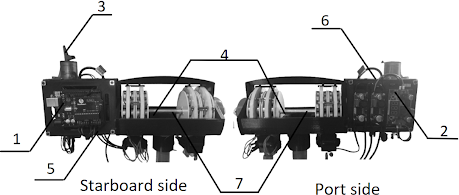
\includegraphics[width=0.45\textwidth]{images/prototype.png}
    \caption{Beta wind turbine prototype. (1) Arduino, (2) port-side buck
        converters, (3) wind vane, (4) power pole connectors, (5) ground busses,
        (6) starboard-side buck converters, and (7) rotor axle.}
    \label{img:prototype}
\end{figure}

Two of the buck converters were damaged from increased voltage during a
high-speed rotor test and were replaced. However, this test confirmed that the
remainder of the system withstood speeds of over \qty{2000}{RPM}.

The computer functionality for the yaw control has been completed and tested.
The turbine blades must be perpendicular to the wind direction to generate the
maximum power. The wind tunnel blows in a single direction, but winds from
different directions can be simulated by rotating the turbine. If the wind is
not blowing directly in front of the turbine, it will rotate itself using a
continuous servo to face the wind. A digital threshold creates a hysteresis
effect to avoid constant adjustments.

In high winds, the yaw control will rotate the turbine to be parallel with the
wind to avoid damage to the turbine blades and potentially harmful excess power
generation, which can cause overheating and fire damage.

\section{Analysis, Modeling, and Simulation Results}

\emph{[TODO]}

\section{Beta Prototype Test Results}
\subsection{Yaw Control}
\label{sec:yaw_control}

For the alpha prototype, the yaw control utilized a 360-degree servo motor to
adjust the turbine's direction based on the wind vane. The servo was not
continuous. Once it reached its maximum rotation, it had to rotate in the
opposite direction. This limitation caused issues if the wind came from near the
servo's maximum or minimum rotational ability. Also, this servo required a 1:1
gear ratio to the nacelle and required a great deal of torque to turn. The
servo utilized was also large and drew excessive power, making it unsuitable
for lower wind speeds.

The new replacement yaw control servo is continuous and draws much less power.
However, the new servo produces less torque and is unable to rotate the
nacelle. The rotation limit is based on the physical wire connection.
Presently, a slip ring mechanism is not used because of the limited requirements
of the Collegiate Wind Competition tests but may be implemented if the twisting
of the wire connections becomes and issue. Unfortunately, even with 3D-printed
gearing and lubrication, the new servo is still unsuitable because it cannot
overcome the static friction on the support.

One possible solution is to add bearings to reduce the friction between the
nacelle and the support. Another solution is to use two of the smaller servos.


\subsection{Load Control}
\label{sec:load_control}

The load control simulation setup consists of a manually-adjustable
\qty{200}{\ohm} rheostat, shown in Figure \ref{img:rheostat}; a Festo four
quadrant dynamometer, with a 2:1 belt transmission pulley ratio coupling
mechanism, shown in Figure \ref{img:dyno}; and the beta prototype shown in
Figure \ref{img:prototype}.

The beta prototype rotor axle is coupled to the dynamometer transmission
axle using a coupling adapter with slip and vibration compensation
capability. The dynamometer is controlled by LabVolt Data Acquisition and
Control Interface software installed on a Windows 10 laptop. The power output
of the system is assessed using the current measuring functionality of an
onboard Precision Digital Current and Power Monitor - INA 260, positioned
at the number 5 callout in Figure \ref{img:prototype}.

The accuracy of the measured current data is verified using a stand-alone Fluke
multimeter. The voltage is measured separately by another independent
multimeter.

\begin{figure}[th]
    \centering
    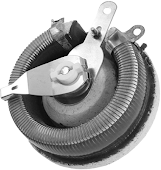
\includegraphics[width=0.2\textwidth]{images/rheostat.png}
    \caption{\qty{200}{\ohm} \qty{0.7}{\A} rheostat}
    \label{img:rheostat}
\end{figure}
\begin{figure}[th]
    \centering
    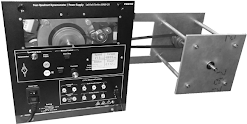
\includegraphics[width=0.45\textwidth]{images/dyno.png}
    \caption{Dynamometer with 2:1 coupling belt transmission ratio mechanism}
    \label{img:dyno}
\end{figure}

During the preparation stage of the analysis, the team determined that the most
useful input parameter would be the torque that the prototype's rotor axle
(shown in Figure \ref{img:prototype}, callout 7) experienced at various wind
speeds. Other input parameters are expressed in terms of this torque. The
mechanical engineering subteam of the Everett Wind Energy Team (EWET)
estimated the torque values, utilizing the fundamental relationships described
in Equation \eqref{eq:torque}:

\begin{equation}
    \label{eq:torque}
    \tau_R = \frac{P_w \times c_p}{\omega_\text{rotor}}
    = \frac{c_p(\lambda, \theta) \times \rho \pi R^3 V_w^2}{2\lambda}
    \text{\,,}
\end{equation}
where $\tau(R)$ is the torque experienced by the prototype rotor axle,
$P(w)$ is the power available in the wind, $C(p)$ is the power-degrading
coefficient expressed as a function of the tip speed ratio and pitch angle,
and $\omega(\text{rotor})$ is the rotational speed of the prototype axle in
(\unit{\radian\per\sec}). For the purpose of the analysis, $C(p)$ was taken to
be \num{0.3}, which indicates that only \qty{30}{\percent} of the power
available in the wind would be extractable. The torque values were assumed to
be between \qty{.1}{\newton\m} and \qty{.3}{\newton\m}. This assumption was
based on previous experiments which demonstrated the approximate range of the
available rotor axle speeds relative to the wind speeds.

Thus torque is used as the input parameter, and generated power is the
output parameter. The load control constants were determined by observing the
Arduino controller operational threshold as one limiting factor and maximum
available power as the other limiting factor. It was determined experimentally
that no more than $\sim$\qty{0.3}{\W} of power was available at
\qty{.1}{\newton\m} constant torque while the Arduino controller was operating.

This result indicates that there is \qty{60}{\mA} of reserve current available
at this torque level for pitch control and data analysis, assuming a
\qty{5}{\V} Arduino supply. At \qty{.3}{\newton\m} torque power output was
measured to be $\sim$\qty{50}{\W}. In this experiment, the rotor's speed was
not captured because it was not a function of the pitch control and tip speed
ratio, which are not available in the dynamometer simulation setup as controlled
parameters.

\subsection{Pitch Control}

During the alpha prototype development, the turbine was tested in the wind
tunnel by manually adjusting the pitch angle of the blades. The pitch control
was designed to control the torque and rotational speed of the rotor to extract
the maximum power from the wind. The team discovered that a steep angle of
attack produced high torque and low rotational speed. Conversely, a shallow
angle of attack produced low torque and higher rotational speed.

The angle of attack will be adjusted by the pitch control mechanism using a
rod that traverses the main shaft of the rotor. The rod will move linearly to
adjust the pitch to a steeper or shallower angle of attack. The particulars of
the mechanism are still being designed. However, the team has decided to
utilize a 180-degree servo to control the pitch angle. Mathematically, the
rotational motion of the servo and the linear motion of the shaft are related
by Equation \eqref{eq:shaft}:

\begin{equation}
    \label{eq:shaft}
    \cos\theta = \text{shaft travel} = \frac{Y}{\tan\theta}
    \text{\,,}
\end{equation}
where the distance $Y$ is the fixed distance of the servo center of rotation to
the shaft and $\theta$ is the angle of the servo.
Figure \ref{img:pitch_control} illustrates the relationship of the servo arm
to the linear shaft motion.

\begin{figure}[th]
    \centering
    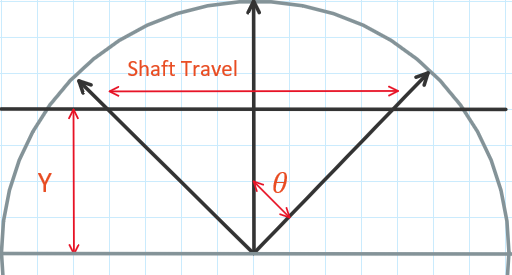
\includegraphics[width=0.45\textwidth]{images/pitch_control.png}
    \caption{Pitch control shaft diagram}
    \label{img:pitch_control}
\end{figure}

An alternative pitch control mechanism is to use a continuous servo with a rack
and pinion to move the shaft. However, the angle of a continuous servo cannot
be determined, only the speed and direction, which would create an open control
loop. Without the angle as a known input, this would require that other inputs,
such as wind and rotor speeds, would be measured after the pitch adjustment to
decide if additional adjustments are required. Reading these additional values
will increase the response time. Therefore, the team decided to use a
traditional non-continuous 180-degree servo.

\subsection{MakerPlot}

MakerPlot is a low-cost Supervisory Control and Data Acquisition (SCADA)
software package\cite{makerplot}. It retreives data and transmits commands over
the serial connection between the Arduino and a laptop computer. EWET has
purchased MakerPlot licenses to be the primary monitoring and manual control
system for the turbine. However, creation of a custom interface is pending on
the completion of the automatic control system and system interface on the
existing Arduinos.

\subsection{Wireless communication}

One limitation of monitoring and controlling the turbine through the Arduino
systems is that wires must run from a laptop into the wind tunnel. To physically
disconnect the system, the addition of a wireless interface utlizing an
ESP32 chip is being explored. The ESP32 has built-in WiFi and Bluetooth Low
Energy, of which Bluetooth is more suitable for the project due to WiFi access
control restrictions that may also be different at the competition venue.

The ESP32 package being utilized is an M5Stack M5StickC Plus. It contains two
buttons, a 1.14 inch OLED display, and both standard female pin connectors and
a Seeed Grove connector. The M5StickC is powered using a USB-C connector with
\qty 5V and \qty{500}{\milli\A}. The unit also contains a built-in
\qty{120}{\milli\A h} battery.

It is possible for the ESP32 to replace one or both of the Arduinos. However,
that would require the purchase of additional external components, such as
motor controllers. It's current task will be limited to being a bridge between
wired serial communications and wireless Bluetooth communications. It will also
be necessary to find a way to read Bluetooth data in at the laptop and have it
appear as though it is coming over the serial port and, conversely, transmit
apparent serial data over Bluetooth instead because MakerPlot only supports
serial communication. A fallback would be to use a second device connected by
USB to the laptop.

\section{Beta Prototype Validation Results}
\subsection{Power Verification Analysis}

Verifying the system's power output is a complex process that depends on the
functionality of the system's controls. The current progress towards
verification as described in Section \ref{sec:load_control}: ``Load Control.''
In summary, the current prototype solution has demonstrated that it will
sustain the predicted power output of the system.

The system has been verified to produce \qty{.3}{\W} of power at
\qty{.1}{\newton\m} of torque and \qty{50}{\W} at \qty{.3}{\newton\m}.

\subsection{Power Quality Analysis}

The Collegiate Wind Competition (CWC) will judge the turbine's power output
quality based on its stability over five seconds. The electrical noise produced
by power electronics switching to manage the system's output is a factor that
must be minimized.

A Digilent Analog Discovery Studio board and associated WaveForms software was
used as an oscilloscope to measure the prototype's power output quality. The
results are shown in Figure \ref{img:osc_voltage} and \ref{img:osc_ripple} in
Appendix \ref{apx:images}. These figures demonstrate that the voltage
fluctuation is within \qty{10}{\percent} of the measured mean voltage
magnitude, and the ripple is \qty{2}{\percent} of the same relative magnitude.
These findings, however, are not indicative of the pass-fail status of the
measured power output, and further clarification is needed of the terms in which
power quality judgments will be passed.

\section{Summary of Work Remaining}
\subsection{Mechanical}

% \emph{[I talk about this in the beta test results section, so this can probably
% be condensed down to just a sentence or so.]}

As discussed in Section \ref{sec:yaw_control}, the yaw control is currently
being revised by the mechanical engineering subteam at EWET. Artemis Project
determined during alpha prototype testing that the existing mechanism was
insufficient to allow the current continuous servo motor to turn the nacelle.
As discussed, a bearing mechanism will be implemented to determine if that
will be sufficient to reduce friction. If not, a second servo motor will be
installed.

The pitch control design is nearing completion. The next stage is to replace
the existing setup with an improved design. Tests will be conducted to
determine the effectiveness of the new pitch control mechanism. The final stage
is to create packaging for the load components to ensure that they are
implemented according to the CWC requirements.


\subsection{Control}

The control subsystem consists of the two Arduino computers (and potential
ESP32), the solid-state relays which control the load, the buck converters
which stabilize and regulate the power output. The Arduinos are connected to
the wind vane to determine wind direction, and Hall sensor on the shaft to
determine the rotational speed. These inputs are used to determine how the
yaw and blade pitch should be adjusted to either maximize power generation
during normal operation or to minimize power and speed in high-wind situations.

The work remaining on the control systems largely depends on the implementation
of the mechanical design. The general algorithms have been developed, although
experimental data is needed with final mechanical design to determine the
magnitude of the adjustments that the computer needs to make.

Although the system is designed to operate autonomously, manual control is
also implemented through the MakerPlot software and an emergency stop button.


\subsection{Programing}

Developing the pitch control software will primarily require the completion and
testing of the physical mechanism to determine the details of what is needed.
Because the 180-degree, non-continuous servo motor was chosen to control the
linear motion of the shaft, preliminary software development can be completed.
The geometry and mechanics of the shaft relative to the servo are known.
However, we do not know how the connections on the other end of the shaft will
affect the rate of change of the pitch. Once the pitch control mechanism has
been implemented, the relationship between the motor and the shaft motion can
be determined experimentally.

The system needs a power pitch control algorithm to improve power generation
stability over a fixed blade design. For the ``power curve performance'' task
of the competition, stable power must be generated at wind speeds from
\qtyrange{5}{11}{\m\per\s}. The buck converters limit the voltage, and the load
controls the current, so producing stable power should not be difficult. Tip
speed ratios for each wind speed have been calculated that would theoretically
produce the most power possible.

The control system must also determine if the tip speed ratio is too high for a
particular load and wind speed in order to avoid stalling. Turbine blades have
a similar shape to an airplane wing, called an airfoil. As with an airplane, a
turbine can suffer a stall. If the angle of attack is too steep, the airflow
can separate from the blade and cause turbulence, pushing the air in the
boundary layer back towards the front of the wing or blade. For an airplane,
this destroys lift, causing the airplane to fall. For a turbine, the rotational
speed will slow significantly. This phenomenon is illustrated in
Figure \ref{img:stall}.

\begin{figure}[th]
    \centering
    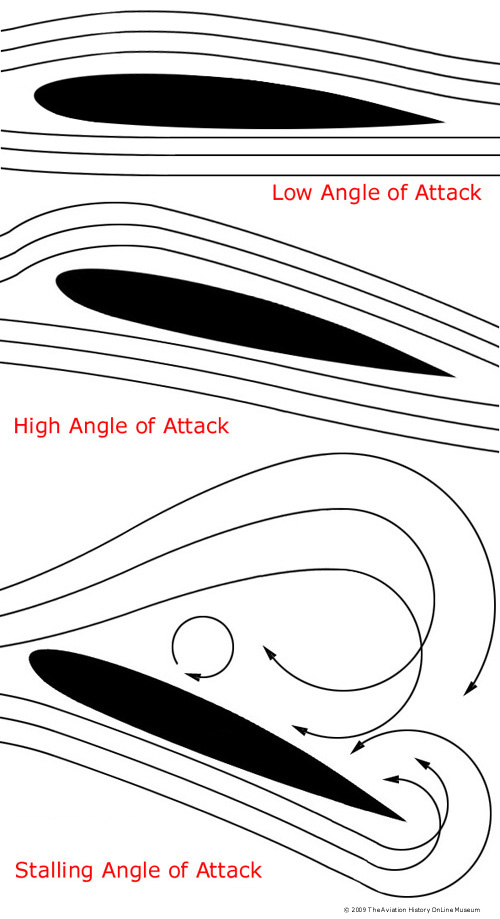
\includegraphics[width=0.3\textwidth]{images/stall.jpg}
    \caption{Airfoil at low angle of attack, high angle of attack, and
        stall\cite{stall}.}
    \label{img:stall}
\end{figure}

It may be wise for the software to position the turbine blade angle for a
more conservative tip speed ratio than calculated to improve stability at the
cost of some output power. This way, the program can have predetermined pitch
angles for each wind speed that can be set and left alone unless prompted
otherwise. Once the desired rotational speed is met, the load will be
increased to the next step.

The durability aspect of the competition requires that the turbine operates at
variable winds speeds from \qtyrange{6}{22}{\m\per\s} for five minutes. The
turbine must be able to produce power across this range.

Artemis Project's primary concern, and the concern in producing an offshore
wind farm in hurricane territory is to keep the turbine's blades from being
damaged or even torn off in a high wind situation. The pitch control system can
adjust the blade's angle of attack to reduce speed and avoid damage in such
cases, in addition to maximizing power output in normal conditions.

However, even when trying to reduce blade rotational speed to protect the
integrity of the turbine, the system must still be able to maintain
consistent power output. With the current KV rating of the turbine, this is
about $1400 \pm 300$\;RPM, which will likely be maintained if we can achieve
low enough tip speed ratios. If low tip speed ratios cannot be achieved
at high wind speeds due to mechanical limitations, blade or
pitch mechanism redesign will be required.


\subsection{Power}

A second Arduino connected to the load will receive commands from the turbine's
Arduino controller and pass them to a bank of solid-state relays. The
Arduino will switch between load resistance values using the onboard
controller. The optimal values will be determined experimentally. Implementing
the software control system will need to wait until the mechanical subteam has
implemented the relay system.

\section{Conclusion}

\emph{[TODO]}
\balance

\raggedright
\printbibliography

\clearpage
\onecolumn
\appendices
\section{Images}
\label{apx:images}

\FloatBarrier
\begin{figure}[th]
    \centering
    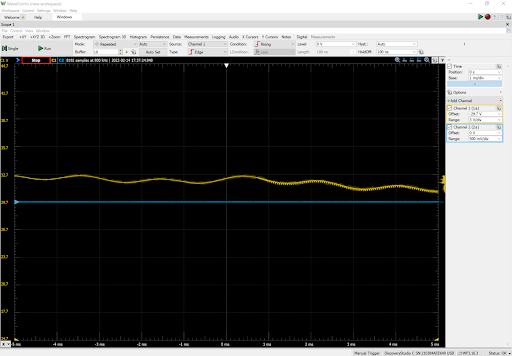
\includegraphics[width=\textwidth]{images/osc_voltage.png}
    \caption{Voltage fluctuation}
    \label{img:osc_voltage}
\end{figure}
\begin{figure}[th]
    \centering
    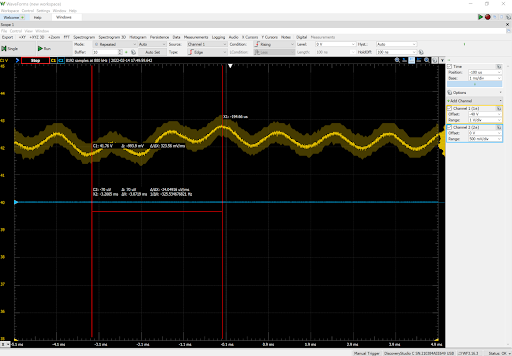
\includegraphics[width=\textwidth]{images/osc_ripple.png}
    \caption{Ripple}
    \label{img:osc_ripple}
\end{figure}

\clearpage
\section{Material Costs}
\label{apx:costs}
\begin{table}[th]
    \centering
    \begin{NiceTabular}{lrl}
        \toprule
        \thead{Product} & \thead{Price (USD)} & \thead{Comment} \\
        \midrule
        \qty{35}{\W} Mini Disc Generator Coreless Generator Three-Phase Permanent &
        \$319.60 & \\
        Rheostat \qty{100}{\W} \qty{100}{\ohm} \qty{1000}{\volt} Std Shaft & \$94.28 & \\
        Rheostat \qty{100}{\W} \qty{200}{\ohm} \qty{1000}{\volt} Std Shaft & \$114.71 & \\
        ALITOVE DC \qty{12}{\V} \qty{5}{\A} Power Supply Adapter Converter Transformer AC & \$11.89 & Unused \\
        MakerPlot licenses & \$236 & \\
        Adafruit 4226 INA260 High or Low Side Voltage, Current, Power Sensor & \$39.80 & Unused (3/4) \\
        Round Tube, 304/304L Stainless Steel, 0.065" Wall Thickness, 5/16" OD & \$13.94 & Research Material \\
        Zener Diodes: \qty{30}{\V} \qty{5}{\W} & \$1.44 & Research Material \\
        Resistors, \qty{25}{\ohm}, \qty{35}{\W}, 5\% & \$6.72 & Research Material \\
        Thick Film Resistors: Through Hole \qty{75}{\ohm} \qty{35}{\W} 5\% TOL & \$6.86 & Research Material \\
        Schottkey Diodes, BOJACK 1N5822, \qty{3}{\A} \qty{40}{\V} DO-201AD & \$5.99 & Replenish WSU stock \\
        MOSFET SMOS Low RON Nch Io: \qty{0.4}{\A} Vdss: \qty{60}{\V} Vgss & \$3.08 & Unused \\
        Potentiometer, Max power \qty{400}{\W} Max R-\qty{200}{\ohm} & \$25.50 & \\
        Mini Electric Linear Actuator Stroke 2 & \$29.99 & Research Material \\
        FEETECH 35KG Continuous Rotation Servo Motor \ang{360} High Torque & \$27.99 & Research Material \\
        DC-DC Buck Boost Converter Module \qtyrange{5.5}{30}{\V} \qty{12}{\V} to \qtyrange{0.5}{30}{\V} & \$25.98 & Research Material \\
        DC\qtyrange{12}{24}{\V} miniature electromagnetic clutch & \$10.25 & Unused \\
        Modern Device Wind Sensor Rev. P & \$24.00 & \\
        DC Buck Converter, DROK DC to DC Step Down Power Supply Module & \$59.98 & \\
        SainSmart 8-Channel \qty{5}{\V} Solid State Relay Module Board for Arduino & \$19.99 & \\
        Misc (connectors, heatshrink tuning, epoxy, PLA str.) & \$89.89 & Manufacturing expense \\
        \midrule
        Total & \$1167.87 \\
        Est. Tax + Shipping (~15\%) &  \$175.18 \\
        Grand Total & \$1343.05 \\
        Total Unused & \$25.21 \\
        Total Research & \$112.92 \\
        \bottomrule
    \end{NiceTabular}
\end{table}

\clearpage
\section{Gantt Chart}
\label{apx:gantt}
\FloatBarrier
\begin{figure}[th]
    \centering
    % \includegraphics[width=\textwidth]{images/gantt-1.png}
\end{figure}
\begin{figure}[th]
    \centering
    % \includegraphics[width=\textwidth]{images/gantt-3.png}
\end{figure}
\begin{figure}[th]
    \centering
    % \includegraphics[width=\textwidth]{images/gantt-4.png}
\end{figure}

\end{document}
